%%%%%%%%%%%%%%%%%%%%%%%%%%%%%%%%%%%%%%%%%
% Journal Article
% LaTeX Template
% Version 1.4 (15/5/16)
%
% This template has been downloaded from:
% http://www.LaTeXTemplates.com
%
% Original author:
% Frits Wenneker (http://www.howtotex.com) with extensive modifications by
% Vel (vel@LaTeXTemplates.com)
%
% License:
% CC BY-NC-SA 3.0 (http://creativecommons.org/licenses/by-nc-sa/3.0/)
%
%%%%%%%%%%%%%%%%%%%%%%%%%%%%%%%%%%%%%%%%%

%----------------------------------------------------------------------------------------
%	PACKAGES AND OTHER DOCUMENT CONFIGURATIONS
%----------------------------------------------------------------------------------------

\documentclass[twoside,twocolumn,10pt]{article}

\usepackage{blindtext} % Package to generate dummy text throughout this template 

\usepackage[sc]{mathpazo} % Use the Palatino font
\usepackage[T1]{fontenc} % Use 8-bit encoding that has 256 glyphs
\linespread{1.05} % Line spacing - Palatino needs more space between lines
\usepackage{microtype} % Slightly tweak font spacing for aesthetics

\usepackage[english]{babel} % Language hyphenation and typographical rules

\usepackage[hmarginratio=1:1,top=32mm,columnsep=20pt]{geometry} % Document margins
\usepackage[hang, small,labelfont=bf,up,textfont=it,up]{caption} % Custom captions under/above floats in tables or figures
\usepackage{booktabs} % Horizontal rules in tables

\usepackage{lettrine} % The lettrine is the first enlarged letter at the beginning of the text

\usepackage{enumitem} % Customized lists
\setlist[itemize]{noitemsep} % Make itemize lists more compact

\usepackage{abstract} % Allows abstract customization
\renewcommand{\abstractnamefont}{\normalfont\bfseries} % Set the "Abstract" text to bold
\renewcommand{\abstracttextfont}{\normalfont\small\itshape} % Set the abstract itself to small italic text

\usepackage{titlesec} % Allows customization of titles
\renewcommand\thesection{\Roman{section}} % Roman numerals for the sections
\renewcommand\thesubsection{\roman{subsection}} % roman numerals for subsections
\titleformat{\section}[block]{\large\scshape\centering}{\thesection.}{1em}{} % Change the look of the section titles
\titleformat{\subsection}[block]{\large}{\thesubsection.}{1em}{} % Change the look of the section titles

\usepackage{fancyhdr} % Headers and footers
\pagestyle{fancy} % All pages have headers and footers
\fancyhead{} % Blank out the default header
\fancyfoot{} % Blank out the default footer
\fancyhead[C]{W266 Final Project $\bullet$ Fall 2019} % Custom header text
\fancyfoot[RO,LE]{\thepage} % Custom footer text

\usepackage{titling} % Customizing the title section

\usepackage{hyperref} % For hyperlinks in the PDF

\usepackage{wrapfig} % 
\usepackage{multirow} % 
\usepackage{threeparttable}
\usepackage{graphicx}
\usepackage{array,booktabs,ragged2e}
\newcolumntype{R}[1]{>{\RaggedLeft\arraybackslash}p{#1}}

%----------------------------------------------------------------------------------------
%	TITLE SECTION
%----------------------------------------------------------------------------------------

\setlength{\droptitle}{-4\baselineskip} % Move the title up

\pretitle{\begin{center}\Large\bfseries} % Article title formatting
\posttitle{\end{center}} % Article title closing formatting
\title{Comparison of Unsupervised Data Augmentation with BERT and XLNet} % Article title
\author{%
\textsc{Thomas P. Goter} \\[1ex] % Your name
\normalsize University of California, Berkeley \\ % Your institution
\normalsize \href{mailto:tomgoter@berkeley.edu}{tomgoter@berkeley.edu} % Your email address
}
\date{\today} % Leave empty to omit a date
\renewcommand{\maketitlehookd}{%
\begin{abstract}
\noindent The Unsupervised Data Augmentation (UDA) methodology \cite{Xie:2019} is further extended beyond its initial use with BERT for use with the XLNet transformer-based neural language model \cite{Yang:2019} for evaluation on a novel text classification dataset. The results discussed herein show that the benefits of UDA are reproducible and extensible to other modeling architectures, namely XLNet. For the novel \textit{Song of Ice and Fire} text classification problem presented herein, absolute error rate reductions of up to 5\% were shown to be possible with an optimized UDA model; however, BERT-based models outperform XLNet based models regardless of UDA.  Additionally, it is shown UDA can achieve the same accuracy as a finetuned model with as little as 67\% of the labeled data. However, UDA is not a magic bullet for enabling the use of complex neural architectures for cases with very limited sets of labeled data, and the complexity of its use and time associated with its optimization should be weighed against the cost of simply labeling additional data.
\end{abstract}
}

%----------------------------------------------------------------------------------------

\begin{document}

% Print the title
\maketitle

%----------------------------------------------------------------------------------------
%	ARTICLE CONTENTS
%----------------------------------------------------------------------------------------

\section{Introduction} \label{introduction}

\lettrine[nindent=0em,lines=3]{T} he state-of-the-art in natural language processing and understanding (NLP/NLU) has been improving at a prodigious pace in the last few years with the development of attention-based neural models \cite{Vaswani:2017} such as BERT \cite{Devlin:2019} and XLNet \cite{Yang:2019}.  While state-of-the-art models are continually being improved, there is still a need in many NLP/NLU tasks to obtain a large set of labeled training data for supervised finetuning.  While this is an obvious observation, it is not necessarily so obvious what can be done when significant amounts of training data are available but much is unlabeled.  This is why the recent work on UDA \cite{Xie:2019} is so exciting; it provides an opportunity to maximize the worth of unlabeled training data through a semi-supervised learning procedure, specifically consistency training.

In \cite{Xie:2019}, UDA was found to be competetive with state-of-the-art, fully supervised neural models for binary text classification problems; however, for multi-class problems the same was not true.  In other words, reducing training data, even when applying UDA, led to significant increases in error rate. The XLNet model \cite{Yang:2019} has been shown to achieve state-of-the-art error rates for multi-class text classification tasks, beating BERT-based models.  However, until this point the UDA methodology has only been coupled with the BERT architecture which was likely state-of-the-art during the development of UDA. Thus, the question of interest is whether UDA when applied to current state-of-the-art model architecture (i.e., XLNet) can
overcome the shortcomings of the BERT-based UDA model for multi-class text classification. The ultimate goals of the work dicussed herein are to quantify, for a five-class text classification task, the following:
\begin{itemize}
	\item Baseline classification performance on novel dataset and how performance varies with labeled data quantity
	\item Finetuned BERT and XLNet performance on the same dataset over the same range of dataset sizes
	\item Reduction in error rate attributable to UDA when using BERT and XLNet based models
\end{itemize}

The dataset chosen for this multi-class text classification task is novel and was derived from the entire volume of the {\it Song of Ice and Fire} (a.k.a. {\it Game of Thrones}) novels by author, George R. R. Martin, and is discussed in more detail in Appendix \ref{data}. This was chosen for two reasons 1) this text was expected to provide a challenging classification dataset due to the presence of many out-of-vocabulary words associated with the rich world created by Martin and 2) the author's personal interest and familiarity with this text.

My contribution to this work is the extension of the UDA methodology to the XLNet model, systematic comparison of BERT and XLNet models for multi-class text classification, and the development and baselining of a new text classification dataset created from the \textit{Song of Ice and Fire} novels.
%------------------------------------------------

\section{Background \& Methods} \label{background}

In this section, the methods for the baseline model, finetuned, fully supervised and UDA models (including data augmentation methodology) are briefly reviewed. A detailed discussion on the comparison between BERT and XLNet model architectures is provided in \cite{Yang:2019}, and a detailed discussion on the UDA methodology is provided in \cite{Xie:2019}. As such, only a brief review is provided herein with specific details on the implementation for the specific classification task.

\subsection{Baseline Model}
The baseline model chosen for this multi-class text classification task was a simple multi-nomial Naive-Bayes model. Unigram and bigram models were evaluated with simple count and tf-idf vectorizers and a grid search to identify the appropriate Laplace smoothing parameters for each case evaluated. This is admittedly a simple model and was chosen as the baseline for three reasons.
\begin{itemize}
 	\item Many of the sequences were assumed to be readily identifiable based on which characters and places appeared in a given sequence. Thus, a simple Naive-Bayes model would likely be effective for these passages.
 	\item Show that the classification task is non-trivial. The baseline was simple enough such that if it achieved high accuracy independent of training set size, the task would have been identified as trivial and a different classification task would have been pursued. As will be shown in Section \ref{results}, this was not the case, and this classification problem is indeed non-trivial. 
 	\item Minimize time spent on developing the baseline model providing opportunities for additional UDA sensitivity studies.
 \end{itemize}

\subsection{Finetuned BERT Model}

The finetuning of a BERT model for text classification is a relatively straightforward task in which pre-trained model parameters are slightly adjusted and the learned embedding for the special [CLS] token is fed to an output layer softmax. The finetuning begins with using learned model parameters from an existing model [4], and weights from all layers are adjusted during the finetuning process. For the sake of this task, the BERT-base, uncased model (12-layer, 768 hidden layer dimension, 12 attention heads and 110M model parameters) has been used as the starting point and was chosen over the BERT-Large model to reduce compute resource requirements for training. The learning rate should be set to avoid "catastrophic forgetting" of the pretrained weights by keeping the learning rate relatively small, but it is treated as a hyperparameter (along with attention and hidden layer dropout rates) during the finetuning process. 

The BERT model uses a special tokenization that includes WordPiece tokenization \cite{Schuster and Nakajima:2012} which breaks words down into smaller pieces and uses special \# tokens to indicate when this word trimming occurs. This helps both with identifying similar root words, but also helps to accomodate out-of-vocabulary words. A brief comparison of tokenization techniques for BERT and XLNet is provided in Appendix \ref{data}. 

Code for the BERT model was leveraged from that used for the original UDA paper [1]; however, it was updated to be compatible with the Google Colaboratory environment to make use of available GPU and TPU resources, Tensorflow 1.15.0 and Python 3. Further the code was integrated with code for XLNet to allow switching between models easily during experimentation. 
\subsection{Finetuned XLNet Model}
Using XLNet for text classification is quite similar to that for BERT. At the time of this analysis, only the cased XLNet models are available for download, and thus was used for this analysis. This model has ~117M parameters and is built on the TransformerXL model architecture \cite{Dai:2019}. As discussed in \cite{Yang:2019}, the XLNet model uses an autoregressive method to estimate a probability distribution of a word given not just its forward or backward context, but with respect to all possible permutations of context for a given sequence. This approach was shown to outperform BERT specifically for text classification making it naturally desirable model to apply to the classification task discussed herein. As with BERT, finetuning is performed by making small adjustments to the pretrained weights for all layers.

 The XLNET model is distributed with an existing SentencePiece model (as BERT is distributed with a vocabulary) which is used for tokenization of sequences. Tokenization differences between models are provided in Appendix \ref{data}.  Finetuning of model weights and hyperparameter tuning (i.e., learning rates, dropout, steps, et cetera) is all achieved with evaluation on the development set. It is noted that while XLNet and BERT models were separately finetuned, optimized hyperparameters were found to be quite similar, with representative values provided in Table \ref{tab:hyper}. These representative values were in most cases found to be optimal for finetuning; however, for the small training set sizes (i.e., 200 and 2000), learning rate and batch size was typically reduced.

 \begin{table}
 	\caption{Comparison of Optimized Hyperparameters}\label{tab:hyper}
 	\centering
 	\resizebox{\columnwidth}{!}{%
 	\begin{tabular}{R{1.2cm}p{1.2cm}p{1.2cm}p{1.2cm}p{1.2cm}p{1.2cm}}
 		\toprule
 		\textbf{Model} & \textbf{Batch Size} & \textbf{Learning Rate} & \textbf{Hidden Layer Dropout} & \textbf{Attention Layer Dropout} & \textbf{Training Steps} \\
 		\midrule
 		\textbf{BERT} & 32 & 3e-5 & 0.15 & 0.10 & 3000 \\
 		\textbf{XLNet} & 32 & 3e-5 & 0.10& 0.10 & 3000 \\
 		\bottomrule
 	\end{tabular}}
 \end{table} 

 
 \subsection{Unsupervised Data Augmentation}
The goal of the work discussed herein was to compare the UDA methodology from \cite{Xie:2019} when coupled with BERT and XLNet models for this {\it Game of Thrones} text classification problem. As such the UDA methodology was kept consistent with that discussed in detail in \cite{Xie:2019}. This is a semi-supervised, consistency training method in which both labeled and unlabeled data is leveraged. In this process a training batch consists of three parts 1) labeled non-augmented examples $E_{L}$, 2) unlabeled, non-augmented examples $E_{U}$, and 3) matching unlabeled, augmented examples $E^{\prime}_{U}$. Standard cross-entropy loss is used on $E_{L}$; however, to this loss term is added the Kullback-Leibler divergence ($D_{KL}$), or relative entropy, between the unlabeled pairs of augmented and non-augmented examples (hence the term consistency training) as shown in Equation \ref{eq:loss}\footnote{Note that the UDA methodology also has tuning parameters such as softmax temperature and confidence threshold masking for the probabilities in the $D_{KL}$ term}. The challenge is performing data augmentation of the unlabeled examples while preserving the expected class label.

 \begin{equation}
 \label{eq:loss}
 Loss_{Total} = -log(q(E_{L})) + -log\frac{q(E_{U})}{q(E^{\prime}_{U})}
 \end{equation}

Two methods for performing this augmentation are discussed in \cite{Xie:2019}, forward-backward translation and TF-IDF word replacement. For the purposes of this analysis only the TF-IDF word replacement augmentation strategy was used. However, in Section \ref{future}, additional text augmentation methods are considered. The TF-IDF word replacement strategy was chosen because it was judged that people and locations would be essentially keywords that would be useful for the book classification task, and this strategy would preserve those. This data augmentation strategy works by generating a TF-IDF score for each word in a given sequence (prior to tokenization). A probability factor is then used to tune the likelihood of each word being replaced, with words having lower TF-IDF scores (relative to the maximum occuring in the sequence) being more likely to be replaced (See Appendix B to \cite{Xie:2019} for more details).  The entire set of  15,001 available training examples is augmented and made available for using during the UDA training process. Additional details along with examples of augmented sequences are provided in Appendix~\ref{data}.

Additional work related to consistency training in none NLP contexts can be found in \cite{Verma:2019} and \cite{Zhang:2019}.

%------------------------------------------------

\section{Analysis Results} \label{results}
Given that the dataset used for the studies discussed herein is novel, baseline accuracy scores were generated and are provided as Figure~\ref{fig:baseline}.   As discussed in Section \ref{background}, the baseline accuracies were generated using a Naive-Bayes (or bag-of-words) approach on the tokenized sequences.  During the baseline model evaluation, the simple CountVectorizer model using bigrams showed superior performance as evaluated on the development set and was thusly used for the final evaluations. Figure~\ref{fig:baseline} clearly shows the expected behavior between accuracy and training set size and motivates the exploration of UDA as a potential means for increasing accuracy when only limited labeled data is available.  Error rates are explicitly given in Table~\ref{tab:errors}. 

\begin{figure}
	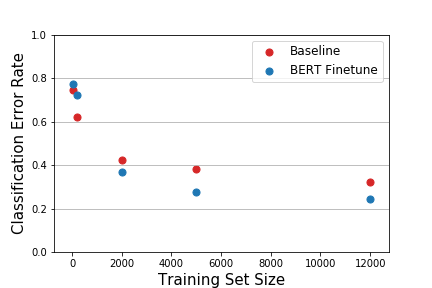
\includegraphics[width=\linewidth]{baseline.png}
	\caption{Baseline Error Rates}
	\label{fig:baseline}
\end{figure}

Finetuned model accuracies are also presented in Table~\ref{tab:errors}, and one can see the clear benefit of the more advanced models, but only with sufficient training data (i.e., $\geq 2000$). With fewer data, the baseline actually outperforms the BERT and XLNet models which is not surprising given the number of parameters in each of these complex models. The tendency to overfit is high given the limited data. Above this level the BERT model is actually highest performing, which was a somewhat surprising result given that XLNet models have been shown to result in state-of-the-art accuracies for text classification \cite{Yang:2019}. It should be noted, however, that the XLNet to BERT multi-class text classification comparison provided in \cite{Yang:2019} was done with only the large models (i.e., with twice as many attention layers).  It is unclear whether the base models showed the same trends as the large models.  In general, the results met with expectation. With the largest training set size, the multi-class error rate approaches 24\%. For the Amazon-5 and Yelp-5 text classification sets, finetuned BERT \cite{Vaswani:2017} and XLNet \cite{Yang:2019} models, 28 and 35\% by comparison.

\begin{figure}
	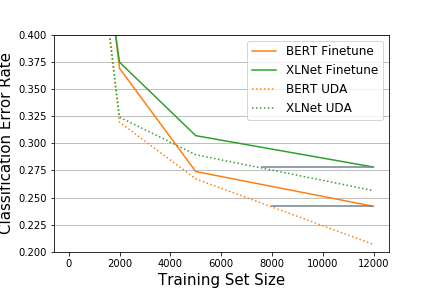
\includegraphics[width=\linewidth]{uda_errors.png}
	\caption{UDA Error Rates}
	\label{fig:uda}
\end{figure}

The analysis results presented in Table~\ref{tab:errors}, show that the application of UDA can provide meaningful error reductions (i.e., between ~1\% and 5\%). Alternatively, if labeled data is limited, this analysis shows that similar levels of accuracy can be achieved even while using ~30\% fewer data as shown by the gray lines on Figure~\ref{fig:uda} between the error rates with 12,000 data without UDA and ~8,000 data (estimated) with UDA applied. With UDA applied, the F1-score of each class is increased and significant underpredictions of classes 2, 3 and 5 are improved, as shown in Figure~\ref{fig:combo}. Unfortunately, UDA was not successful at reducing the error rate of the low data cases (i.e., <2000 labeled examples) to be less than that of the baseline, which indicates some of the limitation of this method relative to adding additional labeled data. Further while there is clearly benefit of applying UDA to the 12,000 dataset size cases, it is unclear that this is coming from adding the additional 3,000 unlabeled examples or whether this benefit could have largely been obtained by simply augmenting the labeled data which would have resulted in a simpler model with fewer hyperparameters.

\begin{figure}
	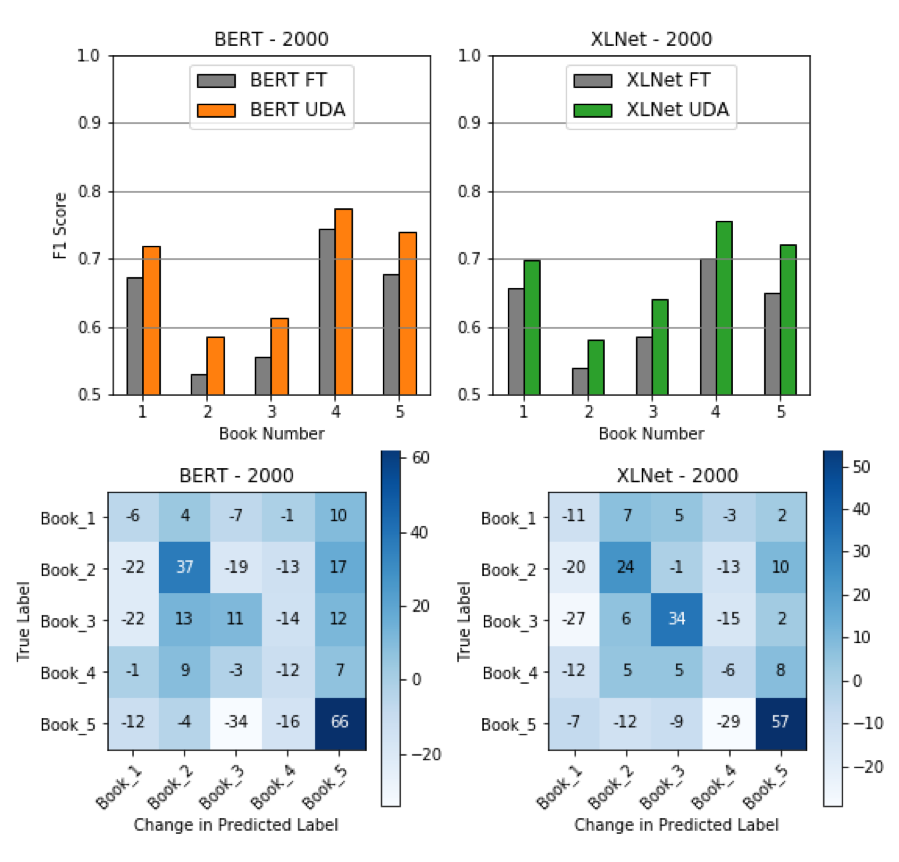
\includegraphics[width=\linewidth]{combo.png}
	\caption{Change in F1 Scores and Predictions with UDA}
	\label{fig:combo}
\end{figure}

\begin{table}
	\resizebox{\columnwidth}{!}{%
	\begin{threeparttable}
	\caption{Classification Error Rates with UDA}\label{tab:errors}
	\centering
		\begin{tabular}{R{1.8cm}p{1.0cm}p{1.0cm}|p{0.6cm}p{0.8cm}p{0.7cm}}
			\toprule
			\multirow{2}{*}\textbf{Model} & \multicolumn{5}{c}{Training Set Size} \\
			\cline{2-6}
			& 20 & 200 & 2000 & 5000 & 12000 \\
			\midrule
			\small
			\textbf{Baseline} & \textbf{0.747} & \textbf{0.622} & 0.422 & 0.382 & 0.322 \\
			\midrule
			\small
			\textbf{BERT FT} & 0.770 & 0.723 & 0.369 & 0.274 & 0.242 \\
			\small
			\textbf{XLNet FT} & \textbf{0.747} & 0.667 & 0.375 & 0.307 & 0.278 \\
			\midrule
			\small
			\textbf{BERT UDA} & 0.776 & 0.676 & \textbf{0.319} & \textbf{0.267} & \textbf{0.207} \\
			\small
			\textbf{XLNet UDA} & 0.818 & 0.676 & 0.324 & 0.289 & 0.256\\
			\bottomrule
			\small
			\textbf{BERT ACE} & -0.006 & 0.047 & 0.045 & 0.007 & 0.035 \\
			\small
			\textbf{BERT RCE} & -0.8\% & 6.5\% & 12.2\% & 2.6\% & 14.5\% \\
			\midrule
			\small
			\textbf{XLNet ACE} & -0.071 & -0.009 & 0.051 & 0.018 & 0.022 \\
			\small
			\textbf{XLNet RCE} & -8.7\% & -1.3\% & 13.6\% & 5.9\% & 7.9\% \\
			\bottomrule
		\end{tabular}
		\begin{tablenotes}
			\small
			\item ACE = Absolute Change in Error
			\item RCE = Relative Change in Error
		\end{tablenotes}
	\end{threeparttable}}
\end{table} 
%------------------------------------------------
\section{Experiments} \label{experiments}
Several experiments aimed at understanding performance tradeoffs with hyperparameters in both the finetuned and UDA models were executed. For finetuning, these studies were focused primarily on batch size, hidden layer dropout rate and learning rate, and all experiments were only evaluated relative to the development set. While other parameters were also studied, these three provided the largest performance changes. An example suite of these senstivities, performed for the XLNet finetuned model are shown in Table~\ref{tab:xlnetft}.

For the semi-supervised portion of this analysis a suite of sensitivity evaluations were run for each training set size to optimize the hyperparameters. The UDA process includes several additional hyperparameters which can make the model optimization process time consuming. Although initial studies were performed following the guidance provided in \cite{Xie:2019}, it was determined that this tuning was quite problem specific. For example, the TF-IDF replacement probability most commonly used in the \cite{Xie:2019} study was stated to be 0.7; however, the studies presented herein optimized at lower replacement probabilities for both BERT and XLNet models, as shown in Figure~\ref{fig:tfidf}\footnote{All other hyperparameters held constant.}.  Further no benefit was observed from either confidence masking or by decreasing softmax temperature (i.e., accentuating probability differences) on the unsupervised data which was another distinction from the work of \cite{Xie:2019}. One common conclusion, however, is the importance of the rate at which labeled data is introduced relative to unlabeled data. This is referred to in \cite{Xie:2019} as training signal annealing (TSA) and discussed in more detail. Selection of the "correct" TSA schedule can be extremely important; during experimentation sensitivity studies evaluating the various TSA schedules showed that simply changing your TSA schedule could double the error rate. Since this is such a large knob for this model, optimization and development of alternate TSA schedules should be considered in future UDA anlayses. For the evaluations with $\geq2000$ data, the logarithmic schedule, which introduces labeled data at the quickest rate, always provided the lowest error rate.

\begin{table}[t]
	\caption{Select XLNet Finetuning Experiments}\label{tab:xlnetft}
	\centering
	\resizebox{\columnwidth}{!}{%
		\begin{tabular}{R{1.2cm}p{1.2cm}p{1.2cm}p{1.2cm}p{1.2cm}}
		\toprule
		Training Set Size & Batch Size & Dropout Rate & Learning Rate & Dev. Error Rate\\
		\midrule
		\textbf{12000} & 32 & 0.10 &3E-5 & \textbf{0.250 }\\
		\textbf{12000} & 32 & \textbf{0.15} &3E-5 & 0.303 \\
		\textbf{12000} & 32 & \textbf{0.20} &3E-5 & 0.353 \\
		\textbf{12000} & \textbf{16} & \textbf{0.15} &3E-5 & 0.389 \\
		\textbf{12000} & 16 & 0.15 &\textbf{5E-5} & 0.377 \\
		\bottomrule
	\end{tabular}}
\end{table} 

\begin{figure}
	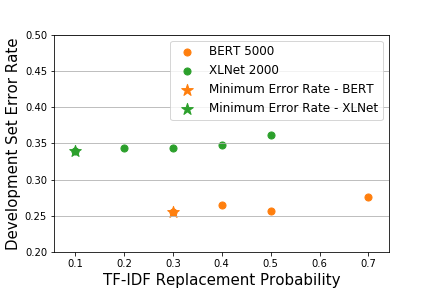
\includegraphics[width=\linewidth]{tfidf.png}
	\caption{TF-IDF Replacement Probability Experiments}
	\label{fig:tfidf}
\end{figure}
%------------------------------------------------

\section{Future Work} \label{future}
The work presented herein only looked at a single data augmentation technique during the UDA application. Future work should evaluate whether the back-translation augmentation methodology applied in \cite{Xie:2019} provides improved performance over the TF-IDF augmentation. Additionally recent work by Sun, et al., \cite{Sun:2019} provides exciting new methods for back-translation by generating a distinct translation from each head in a multi-attention head transformer network. In addition to these alternative data augmentation techniques, the effectiveness of using different TSA schedules for different amounts of training data, seen in \cite{Xie:2019}, was reproduced by this work. Given that these are relatively simple models for how labeled data is introduced during the UDA process, additional work to understand and optimize these schedules should be pursued. In addition to furthering the UDA methodology, additional work should be placed on simplifying the modeling framework used for this analysis. While either model can be run from the same Colaboratory notebook and some elimination of redundant methods was implemented \footnote{ \href{https://github.com/tomgoter/nlp_finalproject}{Project GitHub repository}}, there is still significant streamlining that can be done to enhance simplicity and flexibility.

\section{Conclusions} \label{conclusions}
The analysis presented in this paper has investigated the value of using a semi-supervised learning technique, Unsupervised Data Augmentation \cite{Xie:2019}, using both XLNet and BERT pretrained models for multi-class text classification on the novel \textit{Song of Ice and Fire} dataset. This work represents the first coupling of the UDA methodology with XLNet, and
while the UDA methodology is useful for boosting accuracy, it does not solve the problem of having too few data for training a model. Further the XLNet-based model was outperformed by the BERT-based model across all training set sizes, which was an interesting and unexpected results.  In the text classification task discussed herein, models with fewer than 2000 labeled examples did not outperform the baseline with or without UDA applied. For cases with 2000 or more labeled examples, UDA decreased error rate by up to 5\% absolute and 15\% relative. Prior to future use, the efficiency of applying and optmizing a UDA model should be evaluated relative to the time and cost of simply labeling additional data.
%----------------------------------------------------------------------------------------
%	REFERENCE LIST
%----------------------------------------------------------------------------------------
\begin{thebibliography}{99} % Bibliography 

\bibitem[1] {Xie:2019}
Qizh Xie, Zihang Dai, Eduard Hovy, Minh-Thang Luong and Quoc V. Le. (2019).
\newblock Unsupervised Data Augmentation for Consistency Training.
\newblock {\em arXiv preprint \href{https://arxiv.org/pdf/1904.12848.pdf}{arXiv:1904.12848v4}}, September 2019.

\bibitem[2] {Yang:2019}
Zhilin Yang, Zihang Dai, Yiming Yang, Jaime Carbonell, Ruslan Salakhutdinov, and Quoc V. Le (2019).
\newblock XLNet: Generalized Autoregressive Pretraining for Language Understanding.
\newblock {\em arXiv preprint \href{https://arxiv.org/pdf/1906.08237.pdf}{arXiv:1906.08237v1}}, June 2019.

\bibitem[3] {Vaswani:2017}
Ashish Vaswani, Noam Shazeer, Niki Parmar, Jakob Uszkoreit, Llion Jones, Aidan N. Gomez., Lukasz Kaiser, and Illia Polosukhin (2017).
\newblock Attention is All You Need.
\newblock {\em arXiv \href{https://arxiv.org/pdf/1706.03762.pdf}{arXiv:1706.03762v5}}, December 2017.

\bibitem[4] {Devlin:2019}
Jacob Devlin, Ming-Wei Chang, Kenton Lee, and Kristina Toutanova (2019).
\newblock BERT: Pre-training of Deep Bidirectional Transformers for Language Understanding.
\newblock {\em arXiv \href{https://arxiv.org/pdf/1810.04805.pdf}{arXiv:1810.04805v2}}, May 2019.

\bibitem[5] {Schuster and Nakajima:2012}
Mike Schuster and Kaisuke Nakajima (2012).
\newblock Japanese and Korean Voice Search
 \newblock {\em 2012 IEEE International Conference on Acoustics, Speech, and Signal Processing \href{https://arxiv.org/pdf/1609.08144.pdf}{arXiv:1609.08144}}, 2012.
 
\bibitem[6] {Dai:2019}
Zihang Dai, Zhilin Yang, Yiming Yang, William W Cohen, Jaime Carbonell, Quoc V Le,
and Ruslan Salakhutdinov (2019).
\newblock Transformer-XL: Attentive Language Models Beyond a Fixed-length
 context. 
\newblock {\em arXiv  \href{https://arxiv.org/pdf/1901.02860.pdf} {arXiv:1901.02860v3}}, June 2019.

\bibitem[7]{Sennrich:2016}
Rico Sennrich, Barry Haddow, and Alexandra Birch (2016). 
\newblock Improving Neural Machine Translation Models with Monolingual Data. 
\newblock {\em arXiv \href {https://arxiv.org/pdf/1511.06709.pdf} {arXiv:1511.06709}}, June 2016.

\bibitem[8]{Sun:2019}
Zewei Sun, Shujian Huang, Hao-Ran Wei, Xin-yu Dai and Jiajun Chen. (2019).
\newblock Generating Diverse Translation by Manipulating Multi-head Attention.
\newblock {\em arXiv \href{https://arxiv.org/pdf/1911.09333.pdf}{arXiv:1911.09333v1}}, November 2019.

\bibitem[9]{Verma:2019}
Vikas Verma, Alex Lamb, Juho Kannala, and Yoshua Bengio, and David Lopez-Paz. (2019).
\newblock Interpolation Consistency Training for Semi-supervised Learning.
\newblock {\em arXiv \href{https://arxiv.org/pdf/1903.03825.pdf}{arXiv:1903.03825v3}}, May 2019.

\bibitem[10]{Zhang:2019}
Han Zhang, Zizhao Zhang, Augustus Odena, Honglak Lee. (2019).
\newblock Consitency Regularization for Generative Adversarial Networks.
\newblock {\em arXiv \href{https://arxiv.org/pdf/1911.09333.pdf}{arXiv:1911.09333v1}}, November 2019.
 
\end{thebibliography}
\clearpage
%----------------------------------------------------------------------------------------
\appendix
\onecolumn
\setcounter{table}{0}
\renewcommand{\thetable}{A\arabic{table}}
\renewcommand{\tableformat}{\tablename~\thetable}
\section{Game of Thrones Dataset} \label{data}
The dataset chosen for this multi-class text classification task is novel and was derived from the entire volume of the {\it Song of Ice and Fire} (a.k.a. {\it Game of Thrones}) novels by author, George R. R. Martin. This was chosen for two reasons 1) this text was expected to provide a challenging classification dataset due to the presence of many out-of-vocabulary words associated with the rich world created by Martin and 2) the author's personal interest and familiarity with this text.

The text of the novels was processed by the author and separated into {\it word} sequences\footnote{Tokenization was done after generating training, development and test sets. Thus, the 100 word sequence limit left some room for expected increases in sequence length after tokenization with the BERT or XLNet tokenization processes and minimizing data truncation.} approaching lengths of 100. This length cap was chosen for three reasons 1) provide a significant number of training examples, 2) provide significant context in each training example from which to get value from the BERT and XLNet neural models, and 3) due to hardware limitations, specifically memory, it was expected that tokenized sequences would need to be capped at 128 based on the work discussed in [2] and [4]\footnote{Guidance on sequence length versus GPU/TPU memory availability is provided on the GitHub repositories associated with each of these articles.}. Each sequence was labeled with which book (i.e., 1 through 5) in which is was found. A brief description of the dataset is provided as Table~\ref{tab:data} which indicates there are a total of 19,438 examples in this new dataset. These examples are not evenly spread across the texts, as expected, but balanced subsets were generated for this classification task as discussed below.

\begin{table}[!htb]
	\caption{Descriptive Statistics of Song of Ice and Fire Dataset}\label{tab:data}
	\centering
	\begin{tabular}{p{3.0cm} p{1cm} p{1.5cm} p{3.0cm}}
		\toprule
		Title & Seqs & Median Length & Length Range \\
		\midrule
		{\it Game of Thrones} & 3313 & 86 & [80-146]  \\
		{\it Clash of Kings} & 3608 & 86 & [54-157] \\
		{\it Storm of Swords} & 4575 & 86 & [77-157]  \\
		{\it Feast for Crows} & 3307 & 86 & [74-209]  \\
		{\it Dance with Dragons} & 4635 & 86 & [80-144]  \\
		\midrule
		Totals & 19438 & 86 & [54-209]  \\
		\bottomrule
	\end{tabular}
\end{table}

\begin{table}
	\caption{Division of Dataset}\label{tab:dsets}
	\centering
	\begin{tabular}{R{3.0cm} | R{3cm}}
		\toprule
		\textbf{Dataset} & \textbf{\# of Examples  }\\
		\midrule
		Training  & 15001  \\
		Development  & 2501   \\
		Test  & 1938   \\
		\bottomrule
	\end{tabular}
\end{table}

Data was randomly shuffled and separated into training, development and test sets as shown in Table~\ref{tab:dsets}. Following tokeniziation training data was further subdivided into smaller balanced, labeled subsets of tokenized sequences (e.g., see Table~\ref{tab:tokens}) of  size 20, 200, 2000, 5000, and 12000 for use in various studies discussed in Sections \ref{results} and \ref{experiments}. Further as discussed in Section \ref{background} augmented datasets using all available training data (i.e., 15001 examples) were also generated for the UDA studies.

As noted in Section \ref{background}, there are differences between tokenization between BERT and XLNet models. Some of these differences are the explict (XLNet) versus implict (BERT) treatment of whitespace, the casing, how out-of-vocabulary words get broken down into wordpieces (e.g., p \#\#yl \#\#os and \_Py los for the name "Pylos"), and ordering of special tokens in the sequence and can be seen in Table~\ref{tab:tokens}. Due to the differences in tokenization, separate, tokenized and preprocessed datasets were created for BERT and XLNet models, but these separate datasets contain the same root examples and differ only in tokenization. These preprocessed datasets were stored as TFRecord files for use in the UDA model.

Augmentation of examples was performed using the word replacement strategy discussed in Appendix B to \cite{Xie:2019}.  This procedure calculates a TF-IDF score for every word in each sequence. In a given sequence, words that have the lowest TF-IDF scores are most likely to be replaced, and the probability of replacing any word is scaled by an input hyperparameter.  Examples of augmentated sequences are provided in Table~\ref{tab:augdata} with various scaling factors. From these examples, it can clearly be seen that expected keywords with high TF-IDF values such as the names \textbf{Edd} and \textbf{Sansa} are preserved while things with expected low TF-IDF values, such as punctuation is more likely to be replaced.  

\begin{table}[t]
	\small
	\caption{Tokenization of Examples}\label{tab:tokens}
	\centering
		\begin{tabular}{R{3.0cm}| p{11cm}}
			\toprule
			\textbf{Model} & \textbf{Example} \\
			\midrule
			\textbf{Raw}  & "Is it his fault the old man died? Stannis glanced into the fire.  I never wanted Cressen at that feast. He’d angered me, yes, he’d given me bad counsel, but I did not want him dead.  I’d hoped he might be granted a few years of ease and comfort. He had earned that much, at least, but—he ground his teeth together—but he died. And Pylos serves me ably.  Pylos is the least of it. The letter . . . What did your lords make of it, I wonder?"\\
			\textbf{BERT Tokenization}  &   [CLS] is it his fault the old man died ? stan \#\#nis glanced into the fire . i never wanted cr \#\#ess \#\#en at that feast . he ’ d angered me , yes , he ’ d given me bad counsel , but i did not want him dead . i ’ d hoped he might be granted a few years of ease and comfort . he had earned that much , at least , but — he ground his teeth together — but he died . and p \#\#yl \#\#os serves me ab \#\#ly . p \#\#yl \#\#os is the least of it . the letter . . . what did your lords make of it , i wonder ? [SEP] [PAD] [PAD] [PAD] [PAD] [PAD]\\
			\textbf{XLNet Tokenization}  &  "<unk> <unk> \_I s \_it \_his \_fault \_the \_old \_man \_died ? \_Stan nis \_glanced \_into \_the \_fire . \_I \_never \_wanted \_Cre s sen \_at \_that \_feast . \_He ’ d \_angered \_me , \_yes , \_he ’ d \_given \_me \_bad \_counsel , \_but \_I \_did \_not \_want \_him \_dead . \_I ’ d \_hoped \_he \_might \_be \_granted \_a \_few \_years \_of \_ease \_and \_comfort . \_He \_had \_earned \_that \_much , \_at \_least , \_but — he \_ground \_his \_teeth \_together — but \_he \_died . \_And \_Py los \_serves \_me \_ ably . \_Py los \_is \_the \_least \_of \_it . \_The \_letter \_ . \_ . \_ . \_What \_did \_your \_lord s \_make \_of \_it , \_I \_wonder ? <sep> <cls>"\\
			\bottomrule
		\end{tabular}
\end{table} 

 \begin{table*}[t]
	\small
	\caption{Examples of TF-IDF Data Augmentation}\label{tab:augdata}
	\centering
	\begin{tabular}{p{1.8cm}R{1.5cm} p{11cm}}
		\toprule
		\textbf{Replacement Probability} & \textbf{Data Type} & \textbf{Text}  \\
		\midrule
		
		\multirow{2}{*}{\textbf{p=0.1}} & Original & It was strangely comforting to see Edd’s dour face again\textbf{.} How goes the restoration work? He \textbf{asked} his old steward.\\
		& Augmented & It was strangely comforting to see Edd’s dour face again \textbf{Owen} How goes the restoration work? He \textbf{handled} his old steward.\\
		\midrule
		\multirow{2}{*}{\textbf{p=0.3}} & Original & No\textbf{,} she remembered thinking, \textbf{not} every face, my lord. No one was smiling now. The \textbf{looks} the sparrows gave her were dull, sullen, hostile\textbf{.}\\
		& Augmented & No \textbf{dwell} she remembered thinking, \textbf{worship} every face, my lord \textbf{machines} No one was smiling now. The \textbf{treachery} the sparrows gave \textbf{see} were dull, sullen, hostile \textbf{rooftops}\\
		\midrule
		\multirow{2}{*}{\textbf{p=0.5}} & Original & \textbf{He will,} Sansa \textbf{said,} heart soaring\textbf{. Oh,} I \textbf{know he} will\textbf{. The straw on the floor stank of }urine\textbf{. There was} no \textbf{window}, no bed, \textbf{not even a} slop bucket\textbf{.}\\
		& Augmented & \textbf{Feel} \textbf{falling} \textbf{Quick} Sansa \textbf{custody circle} heart soaring. \textbf{trickle loans} I \textbf{brown shift} will \textbf{crowd priests unadorned stone cleaved roofless narrowed dipped} urine \textbf{Illyrio fleas owns} no \textbf{touch}, no bed, \textbf{congratulate smiling And} slop bucket \textbf{acolytes}\\		
		\bottomrule
	\end{tabular}
\end{table*} 
\end{document}
